\section{Metodologia}

\hspace{0.4cm}Com todos os processos de cálculos definidos, é possível traça-los de forma objetiva para que se chegue da maneira mais simplificada e entendível às perdas de protensão, e fique claro como devem ser programados de forma eficiente na ferramenta computacional. A partir do fluxograma presente na Figura \ref{fig:fluxograma}, é possível compreender esse funcionamento.\bigskip

\begin{figure}[h]
    \centering
    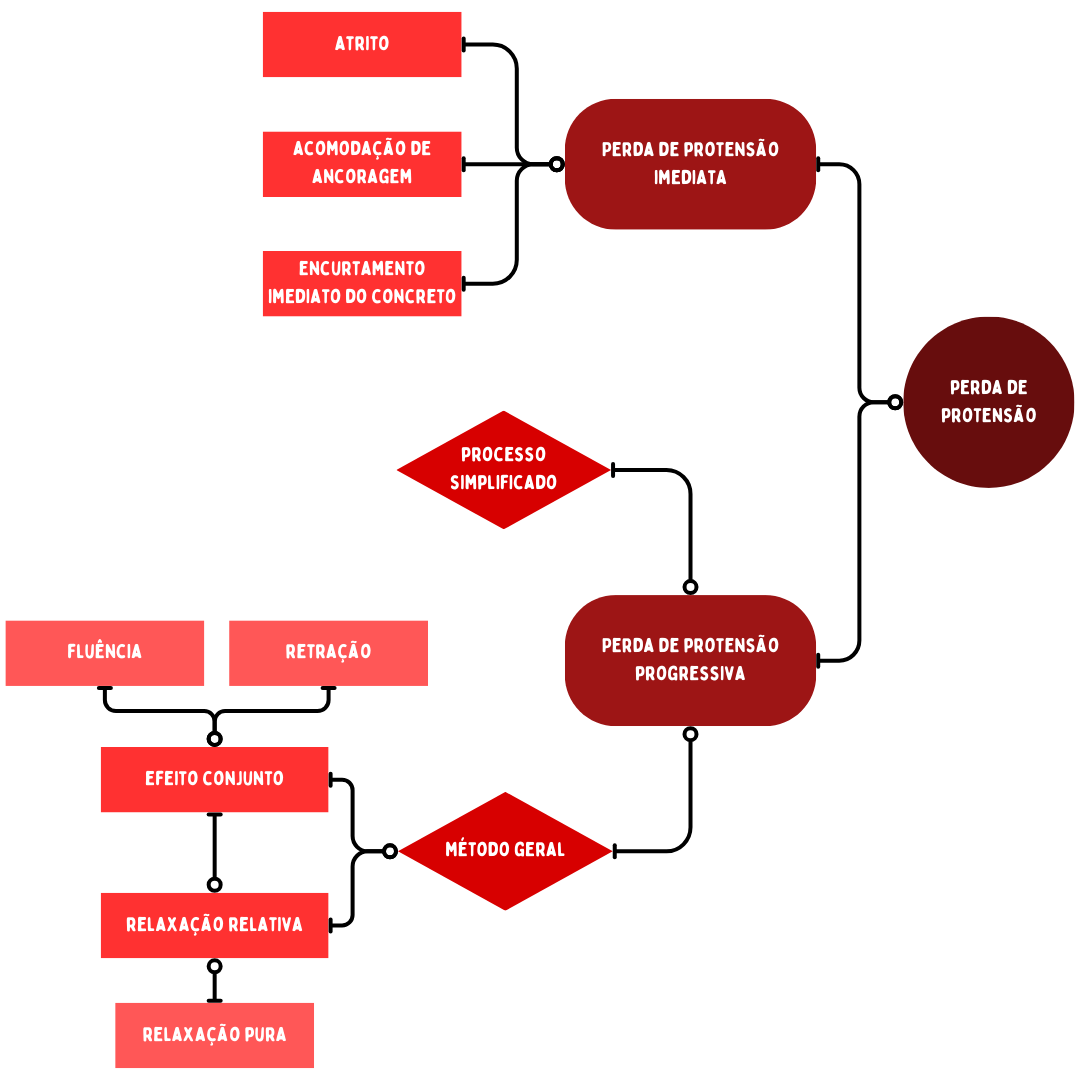
\includegraphics[width=0.9\textwidth]{imgs/fluxograma.png}
    \caption{Fluxograma de cálculo para perda de protensão.}
    \label{fig:fluxograma}
    \medskip
    \small Fonte: Elaboração Própria (2024).
\end{figure}\bigskip

Com todos esses métodos de cálculos da Figura \ref{fig:fluxograma}, é possível construir uma ferramenta que permita ao usuário explorar os processos de cálculo da maneira mais ampla possível, aumentando assim a explicabilidade de seu projeto. Isso posto, a ferramenta foi completamente desenvolvida na linguagem de programação de alto nível \textit{Python} (\citeyear{Py}). Toda sua interface gráfica foi criada a partir da biblioteca nativa da linguagem citada de nome Tkinter (\citeyear{Py}), e as funções para cálculo foram programadas de forma a possibilitar ao usuário chegar à uma perda de protensão final, somando as perdas imediatas com as progressivas.

As funções citadas, para cálculo, foram desenvolvidas seguindo a lógica do fluxograma da Figura \ref{fig:fluxograma}, e os processos expostos anteriormente. Nele é visto que para as perdas imediatas, três tipos de métodos se somam de maneira a compô-la. Já para as perdas progressivas, um entre dois métodos podem ser escolhidos, o processo simplificado que demanda um cálculo mais resumido e simples, com menos explicabilidade, ou o método geral que irá exigir cálculos complementares e mais trabalhosos, com um maior número de variáveis e maior explicabilidade do processo. Com a metodologia escolhida para a perdas de protensão progressivas, soma-se seu resultado com as perdas imediatas resultando na perda de protensão.

É importante entender que cada parte do cálculo das perdas de protensão possuem seu próprio espaço na interface gráfica, além de possuírem funções moduladas e próprias no código fonte para cada método de perda ou cálculo auxiliar. Ela foi pensada e desenvolvida dessa forma, para gerar um maior entendimento do funcionamento da ferramenta e boa capacidade de replicação das funções, junto de uma maior clareza de todo o processo de cálculo que está sendo realizado por trás da interface. Após o desenvolvimento, o código fonte foi disponibilizado em um repositório público (Nóbrega, \citeyear{nobrega}), e foi criado um executável através da biblioteca que transforma códigos \textit{Python} em linguagem de máquinas chamada Pyinstaller (\citeyear{PyI}), e com ele um instalador utilizando-se do Inno \textit{Setup} (\citeyear{IS}), que facilita o empacotamento de arquivos e configurações do programa para o sistema operacional \textit{Windows}.